\section{Energieübertagung}
In diesem Kapitel wird auf das Konzept, die Dimensionierung, die Simulation und den Testaufbau der Energieübertragung eingegangen.

\subsection{Konzept}
Im Gesamtkonzept wird die Schaltung und deren Komponenten erklärt. 

\subsection{Dimensionierung}
In diesen Abschnitt wird die Auslegung der Spule und der Halbleiterelemente erklärt. Für die Dimensionierung der Spule wird die Simulation in femm für den Kopplungsfaktor betrachtet. 

\todo[inline]{Berechnung der Induktivität}
\todo[inline]{Tabelle 10-50kHz}

\todo[inline]{Berechnung MOSFET}

\todo[inline]{Berechnung Ausgangsdiode}

\todo[inline]{Berechnung Snubber Circuit}
\todo[inline]{zwie Möglichkeiten}

\todo[inline]{Berechnung ev. Kondensator}

\subsection{Simulation}
Die Simulation der Schaltung sowie die erhaltenen Erkenntnisse aus der Simulation werden beschrieben.  

\paragraph{FEMM}
\todo[inline]{Infos zu Ferritkern}
\todo[inline]{Erwähnung von Sättigung}

\todo[inline]{Ziel 1: Anzahl Windungen Berechnen}
\todo[inline]{Tabelle Frequenzabhängig, Abstand, Windungen ==> Induktivität}


\todo[inline]{Ziel 2: Kopplungsfaktor Berechnen}
\todo[inline]{Ergebnis für 20, 30, ev. 50kHz}

Um mit FEMM die Selbstinduktion der Primär Spule zu ermitteln, lässt man einen Strom durch die Primär Wicklung und simuliert dies wie in Abbildung. Mit dem simulierten Fluss $ \Psi_{11}  $ und dem Strom $ I_{1} $ kann die Induktivität $ L_{1} $ wie folgt berechnet werden:

\begin{equation}
L_{1}=\frac{\Psi_{11}}{I_{1}}
\label{eq:femm_l1}
\end{equation}

Der Fluss $ \Psi_{1} $ lässt sich in FEMM simulieren in dem man durch die Primär und Sekundär einen Strom laufen lässt, wie in Abbildung. Mit der Formel \ref{eq:femm_M} wird die Gegeninduktivität $ M $ berechnet.

\begin{equation}
M=\frac{\Psi_{1}-\Psi_{11}}{I_{1}}=\frac{\Psi_{12}}{I_{1}}
\label{eq:femm_M}
\end{equation}

Da $ L_{1} $ und $ L_{2} $ den selben Wert besitzen kann man die Formel \ref{eq:kopplungsfaktor} vereinfachen wodurch sich nun der Kopplungsfaktor $ k $ wie folgt definiert:

\begin{equation}
k=\frac{M}{\sqrt{L_{1}^{2}}}
\label{eq:kopplungsfaktor_neu}
\end{equation}

%\begin{figure}
%\centering
%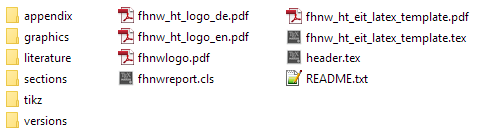
\includegraphics[width=0.8\linewidth]{ordner_struktur.png}
%\caption{FEMM-Simulation mit einem Strom durch die primär Wicklung}\label{fig:FEMM_1}
%\end{figure}


\begin{figure}[t]
	\centering
	\subfloat[Strom durch primär Wicklung.]{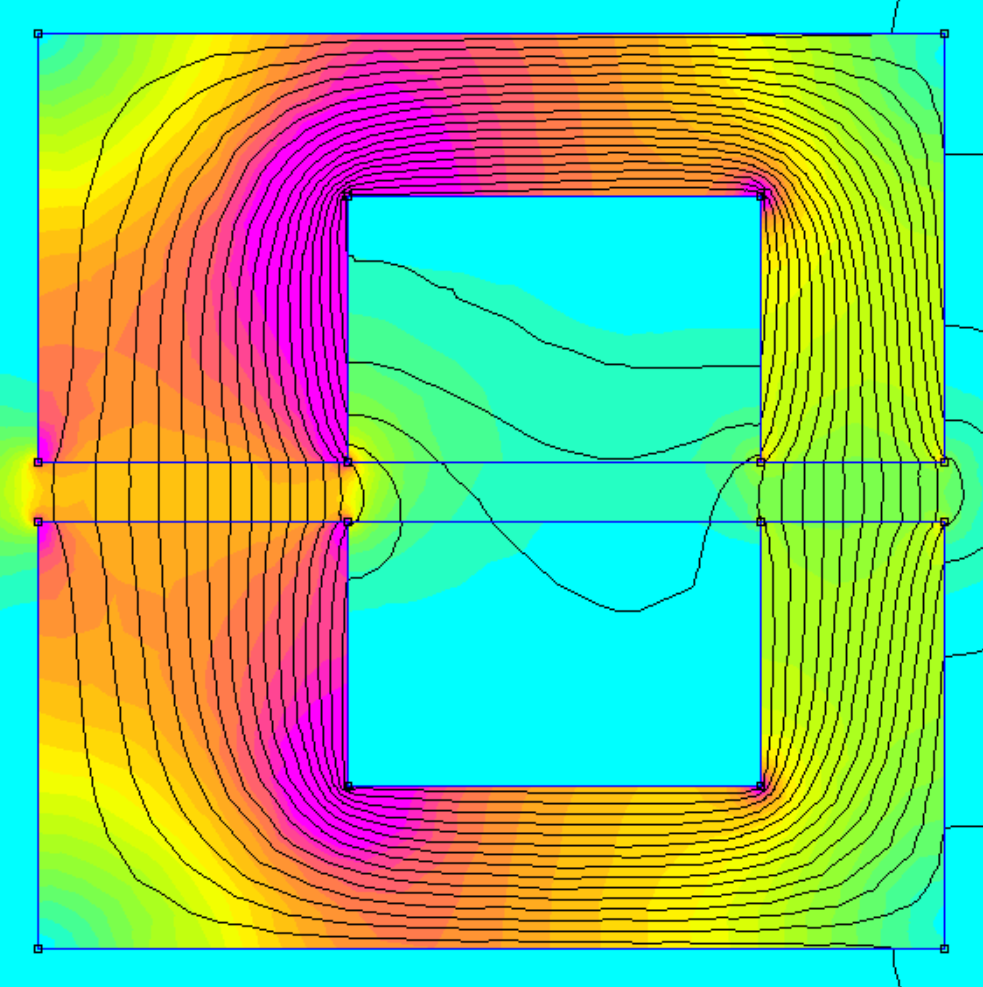
\includegraphics[width=0.45\linewidth]{femm_1.png}}\qquad
	\subfloat[Strom durch primär und sekundär Wicklung.]{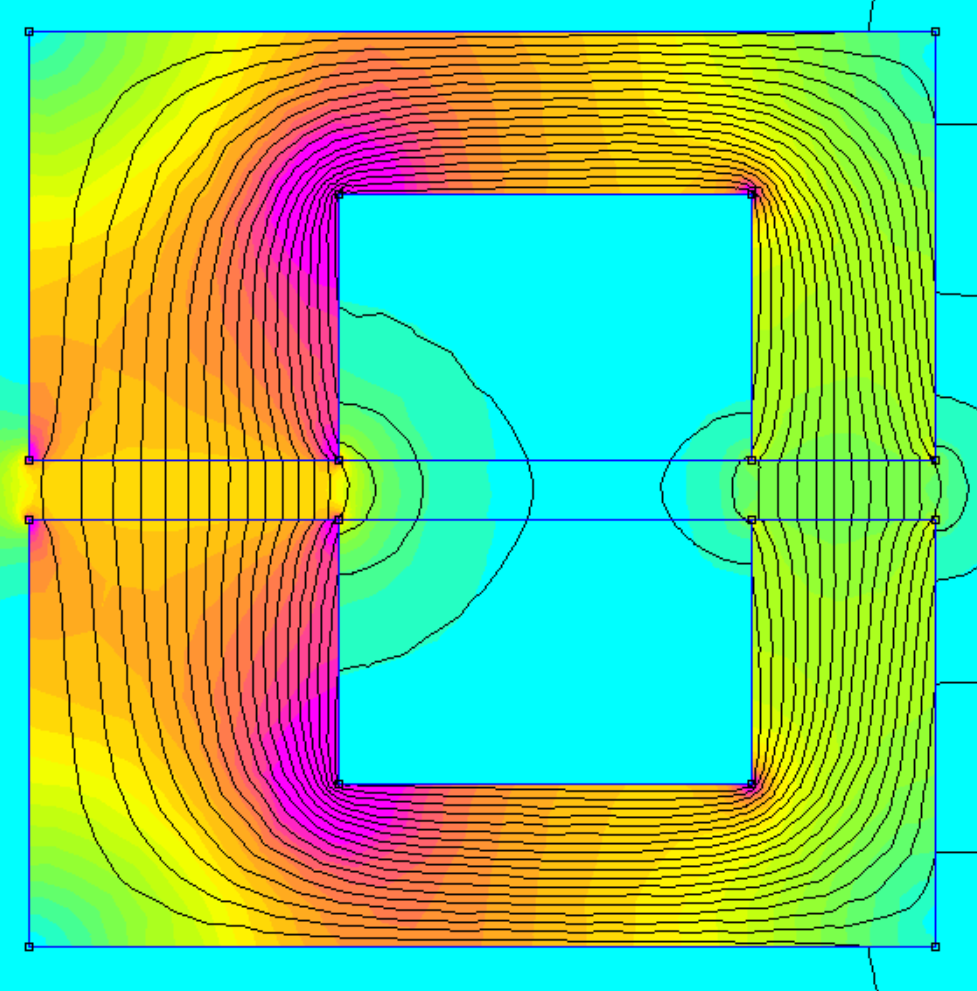
\includegraphics[width=0.45\linewidth]{femm_2.png}}
	\caption{Simulation des FEMM Models.}
	\label{fig:Subfigure}
\end{figure}

\paragraph{Schaltung}
\todo[inline]{Wirkungsgrad}
\todo[inline]{Energie}
\todo[inline]{Strom, Spannung}
\todo[inline]{Aufzeigen von Snubber}
\todo[inline]{Verlustleistung}

\subsection{Testaufbau}
\todo[inline]{Messung Induktivität, Widerstand, Freqeunzabhängig?}

\todo[inline]{Wirkungsgrad}
\todo[inline]{Energie}
\todo[inline]{Strom, Spannung}
\todo[inline]{Aufzeigen von Snubber}
\todo[inline]{Verlustleistung}